\chapter{图的遍历与结构计算}
\label{chap:graph-traversal}

第~\ref{chap:graph-objects}章定义了可达、连通分量、强连通分量、有向无环图、分隔集和同构，这些定义说明了“什么样的结构算数”，却没有说明面对一张存放在计算机里的图，怎样把它们实际找出来。例如，可达性的定义要求“存在一条路径”，而一张图中的路径数目可以随顶点数指数增长，逐条列举路径并不可行。本章研究的问题是：怎样只沿着邻接关系有组织地访问顶点，就得到距离、分量、依赖次序这些结构，并且知道每一项输出为什么正确、花了多少计算。

第~\ref{sec:graph-bfs}节和第~\ref{sec:graph-dfs}节给出两种基本的访问方式。广度优先遍历用队列由近及远逐层推进，输出最少边数和相应路线；深度优先遍历用栈沿一条分支走到底再退回，输出发现与完成两种次序，并能判断有向环。这两种遍历是后面各节共用的工具。第~\ref{sec:graph-connectivity-computation}节用它们计算无向连通分量和生成森林，引入在不断加边时维护分量的并查集，再用两遍深度优先遍历求出有向图的强连通分量；把每个强分量缩成一点得到的图没有有向环。第~\ref{sec:graph-topological-order}节在这样的无环图上安排依赖次序。第~\ref{sec:graph-separator-blocks}节删除一个给定的顶点集，把图拆成若干共享接口的局部块。第~\ref{sec:graph-wl-refinement}节回到同构问题，用邻域信息反复细化顶点标记，得到不依赖编号的比较手段，并指出它的局限。

本章讨论有限图，输入以邻接表给出（第~\ref{sec:graph-representations}节），默认无自环、无平行边，需要保留边身份时另行说明。记顶点数为$n=|V|$；无向图的边数和有向图的弧数都记为$m$，邻接表中无向边在两端各存一次，有向图默认只存出邻居。复杂度中的$O(n+m)$表示所需基本操作次数不超过$n+m$的常数倍。本章的算法只使用结构上的邻接，不比较边权：生成森林只要求连通、不要求总权最小，广度优先遍历只数边数、不计长度。在给定结构中寻找最小成本或最大流量，是第~\ref{chap:graph-optimization}章的问题。

\section{广度优先遍历}
\label{sec:graph-bfs}

从一个起点出发，哪些顶点能够到达，到达每个顶点最少要走几条边，又该沿哪条路线走？按定义逐条检查路径行不通，因为路径数目可能极多。一个更经济的想法是按距离分层推进：先找出起点的全部邻居，它们离起点一条边；再找出这些邻居的尚未见过的邻居，它们离起点两条边；如此继续，直到没有新顶点出现。本节把这个想法写成算法，说明队列怎样保证“先近后远”，并证明算法记录的层数确实是最少边数。

\subsection{广度优先遍历算法}
\label{sec:graph-trav-bfs-algorithm}

\paragraph{需要记录的状态}
按层推进时，要知道哪些顶点已经见过、哪些顶点等待展开、每个顶点在第几层、它是从哪个顶点过来的。于是对起点$s$维护四项状态：发现标记，表示顶点是否已经被找到；一个先进先出的队列$Q$，存放已经发现、但邻居尚未检查的顶点；边数距离$d(v)$；以及\term{父指针}（parent pointer）$p(v)$，记录$v$是从哪个顶点第一次被找到的。初始时只有$s$被发现，$d(s)=0$，$p(s)$为空，队列为$[s]$；其余顶点未发现，距离记为$+\infty$。这种按层访问的过程称为广度优先遍历，也常称\term{广度优先搜索}（breadth-first search，BFS）。

\begin{algorithm}[广度优先遍历]
\label{alg:graph-trav-bfs}
输入：图$\mathcal G=(V,E)$的邻接表，起点$s\in V$。输出：距离$d(v)$与父指针$p(v)$，$v\in V$。
\begin{enumerate}
  \item 标记$s$为已发现，置$d(s)=0$、$p(s)$为空，令$Q=[s]$；其余顶点未发现，$d(v)=+\infty$。
  \item 当$Q$非空时，取出队首$u$，按邻接表依次读取$u$的邻居$v$（有向图只读出邻居$v\in N^+(u)$）。若$v$未发现，立即标记$v$为已发现，置$d(v)=d(u)+1$、$p(v)=u$，并把$v$放到队尾；若$v$已发现，跳过。
  \item 队列为空时停止。
\end{enumerate}
\end{algorithm}

标记必须在入队时完成，而不是等到出队时。两个已发现的顶点可能共享一个尚未发现的邻居；若出队时才标记，这个邻居会被两个顶点各放入队列一次，距离和父指针也可能被改写。入队即标记保证每个顶点至多入队一次。

\paragraph{贯穿图上的队列轨迹}
在第~\ref{sec:graph-basic-concepts}节的贯穿四点图上，以$1$为起点，并约定按编号从小到大读取邻居。图~\ref{fig:graph-trav-bfs-queue}(b)逐行列出了每次出队后的队列。取出$1$时发现$2,3$，队列变为$[2,3]$；取出$2$时，邻居$1,3$都已发现，只有$4$是新的，队列变为$[3,4]$；取出$3$时，邻居$1,2,4$全部已发现，$4$不会第二次入队；最后取出$4$，队列为空。结果是$d(2)=d(3)=1$、$d(4)=2$，父指针为$p(2)=p(3)=1$、$p(4)=2$。图~\ref{fig:graph-trav-bfs-queue}(a)把各顶点按$d$值分到三层，蓝色箭头就是父指针所指的边。

\begin{figure}[!htb]
  \centering
  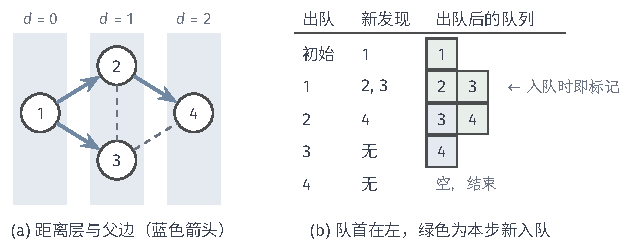
\includegraphics[width=106.7mm]{figures/01-basic-mathematics/04-graphs/tikz/c2-bfs-queue-trace/figure.pdf}
  \caption{贯穿四点图上从顶点$1$出发的广度优先遍历，邻居按编号递增读取。(a)顶点按边数距离$d$分为三层，蓝色箭头是父指针对应的边，虚线是检查过但没有带来新顶点的边。(b)每次出队后的队列，队首在左，绿色格子是这一步新入队的顶点；取出$3$时$4$已在队中，不再重复入队。}
  \label{fig:graph-trav-bfs-queue}
\end{figure}

\paragraph{由父指针恢复路线}
父指针给出的是一条实际路线，而不只是一个距离数值。要得到从$s$到已发现顶点$t$的路线，从$t$出发反复取父指针，直到回到$s$，再把得到的顶点序列反转。在上例中，$4$的父指针是$2$，$2$的父指针是$1$，反转后得到路线$1\to2\to4$，恰有$d(4)=2$条边。父指针总是指向更早发现的顶点，所以沿父指针回溯不会绕圈，一定在有限步内回到$s$。若$t$始终未被发现，即$d(t)=+\infty$，算法应报告$t$从$s$不可达，而不能输出任何路线。

路线并不唯一。若把邻居的读取次序改为先读$3$再读$2$，那么取出$1$后队列为$[3,2]$，$4$会在展开$3$时被发现，父指针变成$p(4)=3$，路线变成$1\to3\to4$。两条路线不同，但边数都是$2$。下面的定理说明，改变同层顶点的处理次序可能改变父指针，却不会改变距离。

\subsection{正确性与计算开销}
\label{sec:graph-trav-bfs-correctness}

\paragraph{为什么首次记录就是最少边数}
记$\operatorname{dist}(s,v)$为从$s$到$v$的路径的最少边数，不可达时为$+\infty$。算法只在顶点第一次被发现时写入$d(v)$，以后不再修改。我们要说明，这个“第一次”恰好发生在最短的距离上。

\begin{theorem}[广度优先遍历的距离]
\label{thm:graph-trav-bfs-distance}
设对有限图$\mathcal G$和起点$s$执行算法~\ref{alg:graph-trav-bfs}。则对每个顶点$v$，$d(v)=\operatorname{dist}(s,v)$；当$v$可达时，沿父指针从$v$回到$s$的路线恰有$d(v)$条边。
\end{theorem}

\begin{proof}
先说明$d(v)$不会小于真实距离。若$d(v)$有限且$v\neq s$，则$d(p(v))=d(v)-1$，沿父指针每退一步距离减一，$d(v)$步后回到$s$。反转这串顶点就得到一条从$s$到$v$、恰有$d(v)$条边的路线，所以$d(v)\geq\operatorname{dist}(s,v)$。

再说明队列中的距离值有一个固定的形状：从队首到队尾不减，且最大值与最小值至多相差$1$。初始队列只有$s$，满足这一点。设某时刻队列中的值为若干个$k$后接若干个$k+1$，取出的队首$u$有$d(u)=k$，新加入的顶点距离都是$k+1$，并放在队尾，形状仍然保持。由此可知，顶点出队时的距离值按时间不减。

最后对$\delta=\operatorname{dist}(s,v)$归纳，证明有限距离的顶点都会被发现且$d(v)\leq\delta$。$\delta=0$时$v=s$。设$\delta\geq1$，并设距离小于$\delta$的顶点都已满足结论。取一条从$s$到$v$的最短路径，记其倒数第二个顶点为$x$，则$\operatorname{dist}(s,x)=\delta-1$，由归纳假设$x$被发现且$d(x)=\delta-1$。$x$入过队，就一定在某一时刻出队并检查邻居$v$。若此时$v$尚未发现，就得到$d(v)=d(x)+1=\delta$；若$v$已经被发现，则发现它的顶点$u$出队不晚于$x$，按上一段的单调性$d(u)\leq d(x)$，于是$d(v)=d(u)+1\leq\delta$。两个方向合起来得到$d(v)=\operatorname{dist}(s,v)$。不可达的顶点没有任何从$s$出发的路线，第一段说明它不可能得到有限的$d$值。
\end{proof}

证明的关键是第二段的队列形状：算法处理第$k$层时，只会首次发现第$k+1$层的顶点；第$k+1$层的顶点全部排在第$k$层之后。倒数第二个顶点$x$比$v$少一层，一定先被展开，因此$v$不可能等到更远的层才被发现。

\paragraph{计算开销}
以邻接表存储时，每个顶点至多入队一次、出队一次；每个顶点出队时把它的邻接表读一遍，因此每条邻接记录只被检查常数次。无向图的邻接记录共$2m$条，有向图的出邻接记录共$m$条，所以总时间为$O(n+m)$。发现标记、距离、父指针和队列各占$O(n)$额外空间。这一结论依赖“列出邻居的代价与度数成正比”。若图以邻接矩阵存储，找出一个顶点的邻居要扫描矩阵的一整行，$n$个顶点共扫描$n^2$个位置，时间变为$O(n^2)$；对稀疏图，这比$O(n+m)$大得多。

\paragraph{最少边数不是最小总长度}
广度优先遍历把每条边都算作一步。边上带有长度时，边数最少的路线不一定总长度最小。图~\ref{fig:graph-trav-bfs-weighted}中，从$s$直接到$t$只需一条边，广度优先遍历就会用这条边记录$t$，但它的长度是$5$；经过$a$的路线多走一条边，总长度却只有$1+1=2$。所以广度优先遍历只解决所有边长相等时的最短路问题。一般边长下的最短路需要比较累计长度，留到第~\ref{sec:graph-shortest-paths}节。

\begin{figure}[!htb]
  \centering
  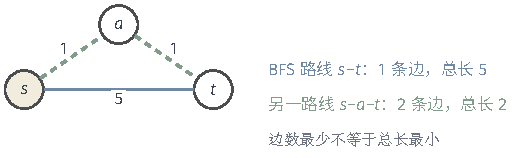
\includegraphics[width=87.8mm]{figures/01-basic-mathematics/04-graphs/tikz/c2-bfs-weighted-counterexample/figure.pdf}
  \caption{带权反例。边旁数字是长度。广度优先遍历从$s$出发时经直接边一步发现$t$（蓝色），这条路线总长$5$；绿色虚线路线$s\text{--}a\text{--}t$多一条边，总长只有$2$。广度优先遍历最小化的是边数，不是总长度。}
  \label{fig:graph-trav-bfs-weighted}
\end{figure}

此外，一次广度优先遍历只覆盖从$s$可达的部分。遍历结束时距离仍为$+\infty$的顶点没有被访问，不能据此断言它们是孤立点，它们之间可能有很多边。要给全图的每个顶点划分连通分量，需要在外层不断换新的起点重新启动，这是第~\ref{sec:graph-connectivity-computation}节的内容。

\subsection{多源广度优先遍历}
\label{sec:graph-trav-multi-source-bfs}

\paragraph{从一组起点同时出发}
有时关心的不是离某一个起点有多远，而是离一组起点中最近的那个有多远。例如在网格上放置若干个种子，问每个格子离最近的种子几步。给定起点集合$S\subseteq V$，定义
\[
\operatorname{dist}(S,v)=\min_{s\in S}\operatorname{dist}(s,v),
\]
空集上的最小值约定为$+\infty$。做法是把$S$中所有顶点同时作为第$0$层：初始时它们都被标记、距离为$0$、父指针为空，并按任意次序全部放入队列，此后完全按算法~\ref{alg:graph-trav-bfs}执行。这称为\term{多源广度优先遍历}（multi-source breadth-first search）。

为什么这样得到的是到最近起点的距离？设想添加一个新顶点$s^*$，从它向$S$中每个顶点连一条边（有向图中连弧$s^*\to s$）。在新图中，任一顶点$v\notin\{s^*\}$满足$\operatorname{dist}(s^*,v)=1+\operatorname{dist}(S,v)$，因为从$s^*$出发的路线第一步必然进入$S$中的某个点。从$s^*$做普通广度优先遍历，第一次出队就把$S$中所有顶点以距离$1$放入队列，此后的过程与多源版本完全相同，只是所有距离多了$1$。由定理~\ref{thm:graph-trav-bfs-distance}即得多源版本输出$\operatorname{dist}(S,v)$，而且沿父指针回溯会停在某个起点上，它就是离$v$最近的起点之一。

\paragraph{网格上的种子传播}
图~\ref{fig:graph-trav-multi-source}是一个$3\times5$网格，相邻格子以上下左右相连，中间一个格子不属于图。两个起点放在左上角和右下角，每个格子中的数字是它到较近起点的边数。例如第一行第四个格子离左上角$3$步、离右下角$3$步，记为$3$；第一行最右的格子离右下角只有$2$步，记为$2$。若只从左上角出发，右下角的格子距离为$6$。

\begin{figure}[!htb]
  \centering
  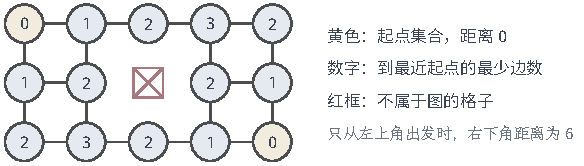
\includegraphics[width=99.0mm]{figures/01-basic-mathematics/04-graphs/tikz/c2-multi-source-bfs/figure.pdf}
  \caption{$3\times5$网格上的多源广度优先遍历。网格以上下左右相邻连边，红框格子不属于图；两个黄色起点同时作为第$0$层。每个顶点中的数字是到较近起点的最少边数，所有距离由一次遍历得到。}
  \label{fig:graph-trav-multi-source}
\end{figure}

\paragraph{与逐个起点遍历的区别}
多源遍历与“对每个起点各做一次广度优先遍历”回答的是不同问题。后者得到$|S|$组距离，能说出$v$到每一个起点各有多远，需要$O(|S|(n+m))$时间；多源遍历只给出到最近起点的距离及对应的起点，一次遍历只需$O(n+m)$时间。若$S$为空，队列一开始就为空，所有顶点保持未发现，输出的可达集为空集，这与$\operatorname{dist}(\varnothing,v)=+\infty$的约定一致。图像中从种子出发的区域生长是这一机制的典型用途；判断哪些像素属于前景、怎样选择邻接规则等完整处理留到应用部分。

\section{深度优先遍历}
\label{sec:graph-dfs}

广度优先遍历同时推进许多条路线，每条只走一步。另一种访问方式是只盯住一条路线：从当前顶点走向一个尚未见过的邻居，再从那里继续往前，直到无路可走才退回上一个顶点，改走它的下一个邻居。走迷宫时用左手扶墙一路前进、碰到死路再折回，就是这种方式。它天然地维持着“当前正在走的这条分支”，因而能判断沿当前分支是否绕回了自己，也能记录每个顶点何时把所有出路都探完。本节建立这一过程，并说明这两条信息分别有什么用。

\subsection{栈与递归访问}
\label{sec:graph-trav-dfs-stack}

\paragraph{三种状态与栈帧}
沿分支前进时，一个顶点经历三个阶段：尚未被走到，称为未发现；已经走到、但它的邻居还没有检查完，称为处理中；邻居全部检查完毕、不会再从它出发，称为已完成。区分后两种状态是必要的，因为“已经见过”并不等于“已经处理完”。处于处理中的顶点恰好构成从本次起点到当前位置的一条分支，用一个后进先出的栈保存：栈底是起点，栈顶是当前顶点。

只记住栈中的顶点还不够。退回到某个顶点时，需要接着检查它的下一个邻居，而不是从头再来。因此栈中的每一帧保存一个顶点$u$，以及$u$的邻接表中下一条待检查记录的位置。另外用父指针$p(v)$记录$v$是从哪个顶点走过来的。这种访问方式称为深度优先遍历，也常称\term{深度优先搜索}（depth-first search，DFS）。

\begin{algorithm}[深度优先遍历（显式栈）]
\label{alg:graph-trav-dfs}
输入：图$\mathcal G=(V,E)$的邻接表。输出：父指针、每个顶点的发现时刻$d(v)$与完成时刻$f(v)$。
\begin{enumerate}
  \item 所有顶点置为未发现，时钟$t=0$。按某个固定次序扫描顶点；每遇到一个未发现的顶点$r$，令$p(r)$为空，执行下面两步。
  \item 发现$r$：$t\gets t+1$，$d(r)=t$，$r$改为处理中，把帧$(r,\text{邻接表起点})$压入栈。
  \item 当栈非空时，看栈顶帧$(u,\text{位置})$。若$u$还有未检查的邻居，读取下一个邻居$v$（有向图只读出邻居），并把位置后移一格：$v$未发现时，置$p(v)=u$，$t\gets t+1$，$d(v)=t$，$v$改为处理中并压入新帧；$v$处于处理中或已完成时，不压栈，继续下一轮。若$u$的邻居已全部检查，则$t\gets t+1$，$f(u)=t$，$u$改为已完成并弹出栈顶帧。
\end{enumerate}
\end{algorithm}

用递归写，同样的过程更短：访问$u$时先记发现时刻，然后对每个未发现的邻居$v$置$p(v)=u$并递归访问$v$，所有邻居处理完后记完成时刻。递归调用时，程序运行时会自动保存“$u$检查到了第几个邻居”，这正是显式栈中每一帧记录的位置。两种写法的访问次序完全一样。

\paragraph{完整执行过程}
图~\ref{fig:graph-trav-dfs-stack}(a)是一个有分支的有向图，弧为$1\to2$、$1\to5$、$2\to3$、$2\to4$、$5\to4$。从$1$出发并按编号读取出邻居：发现$1$，再发现$2$，再发现$3$；$3$没有出邻居，于是完成$3$并弹栈，回到$2$。$2$的下一个出邻居$4$未发现，压栈；$4$也没有出邻居，完成后回到$2$，此时$2$的邻居已检查完，完成$2$。回到$1$，它的下一个出邻居$5$未发现，压栈；$5$唯一的出邻居$4$已经完成，不再压栈，$5$随即完成；最后完成$1$，栈变空。图~\ref{fig:graph-trav-dfs-stack}(b)画出了每个事件之后的栈，黄色格子是栈顶。

\begin{figure}[!htb]
  \centering
  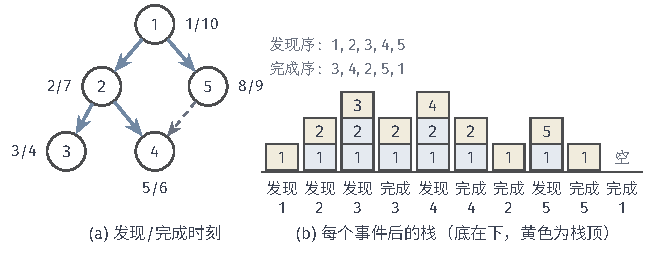
\includegraphics[width=109.8mm]{figures/01-basic-mathematics/04-graphs/tikz/c2-dfs-stack-trace/figure.pdf}
  \caption{有向图$1\to2$、$1\to5$、$2\to3$、$2\to4$、$5\to4$上从$1$出发的深度优先遍历，出邻居按编号读取。(a)顶点旁的“$d/f$”是发现时刻与完成时刻，蓝色箭头是父指针对应的弧，虚线弧$5\to4$检查时$4$已完成。(b)十个事件后的栈，底在下、栈顶为黄色；栈高上升对应发现，下降对应完成。}
  \label{fig:graph-trav-dfs-stack}
\end{figure}

若栈空时仍有未发现的顶点，算法回到第一步，从下一个未发现顶点重新开始。已经完成的顶点保持原状态，不会被重新访问。这样，整次执行把每个顶点恰好发现一次、完成一次；父指针把顶点组织成若干棵有根树，称为深度优先森林。只在发现时处理顶点，得不到“何时探完”的信息，因此完成事件要单独记录，下一小节会看到它的用处。

\paragraph{计算开销}
每个顶点恰好压栈一次、弹栈一次；每一帧的位置只向后移动，所以每条邻接记录恰好被读取一次。邻接表下总时间为$O(n+m)$，状态、时刻、父指针和栈占$O(n)$额外空间。栈的深度等于当前分支上的顶点数，最坏可达$n$：在一条长链$1\to2\to\cdots\to n$上，栈会一直增长到装下全部顶点。递归实现时，这意味着递归深度也是$n$，可能超出程序运行环境允许的调用深度；显式栈把这部分存储放在普通数组中，避免这一问题。

\subsection{发现次序与完成次序}
\label{sec:graph-trav-dfs-orders}

\paragraph{两种次序}
按发现时刻从小到大排列顶点，得到\term{发现次序}（discovery order）；按完成时刻排列，得到\term{完成次序}（finishing order）。在图~\ref{fig:graph-trav-dfs-stack}中，发现次序是$1,2,3,4,5$，完成次序是$3,4,2,5,1$。两种次序的差别来自栈的结构：一个顶点被发现之后，在它弹栈之前压入的所有顶点都位于它上方，必须先弹出。所以一个顶点的后代全部先于它完成，而它自己最后完成；$2$的后代$3,4$先完成，然后才轮到$2$。

下面两个引理把这一观察写准确。第一个说明时刻区间怎样嵌套，第二个说明哪些顶点一定会成为后代；第~\ref{sec:graph-connectivity-computation}节计算强连通分量、第~\ref{sec:graph-topological-order}节构造拓扑次序时都要用到它们。

\begin{lemma}[时刻区间的嵌套]
\label{lem:graph-trav-dfs-nesting}
在一次完整的深度优先遍历中，若顶点$v$在$u$处于处理中时被发现，即$d(u)<d(v)<f(u)$，则$v$是$u$在深度优先森林中的后代，且$f(v)<f(u)$。
\end{lemma}

\begin{proof}
$v$被发现时压入栈，位于$u$的上方，因为此时$u$仍在栈中。栈后进先出，$v$必须在$u$之前弹出，所以$f(v)<f(u)$。另外，$v$的父指针指向发现它时的栈顶，这个栈顶要么是$u$，要么是在$u$之后压入的顶点；对后者重复同样的推理，父指针链只会经过$u$上方的顶点，最终到达$u$。因此$v$是$u$的后代。
\end{proof}

\begin{lemma}[未发现路径]
\label{lem:graph-trav-white-path}
若在时刻$d(u)$存在一条从$u$到$v$的路径（有向图中沿弧方向），路径上除$u$以外的顶点此时都未发现，则$v$最终成为$u$的后代，从而$f(v)<f(u)$。
\end{lemma}

\begin{proof}
假设结论不成立，在路径上取第一个不成为$u$后代的顶点$w$，记它在路径上的前一个顶点为$x$。$x$是$u$本身或$u$的后代，所以$f(x)\leq f(u)$。$x$在完成之前要检查弧$x\to w$，因此$w$在$f(x)$之前已被发现；而按假设$w$在$d(u)$时尚未发现，所以$d(u)<d(w)<f(x)\leq f(u)$。由引理~\ref{lem:graph-trav-dfs-nesting}，$w$是$u$的后代，矛盾。
\end{proof}

\paragraph{共享后继：发现次序不能代替完成次序}
设图~\ref{fig:graph-trav-dfs-stack}中的弧表示依赖，$i\to j$意味着$i$要排在$j$之前。顶点$4$同时是$2$和$5$的后继。若按发现次序$1,2,3,4,5$安排，$5$排在$4$之后，违反了弧$5\to4$：发现$4$时走的是经过$2$的分支，发现次序完全没有反映$5$也指向它。完成次序则不同。$4$在$5$之前就已完成，反转完成次序得到$1,5,2,4,3$，逐条检查五条弧都是起点在前。第~\ref{sec:graph-trav-dfs-toposort}节会证明，在无环图中这一做法总是成立。

\paragraph{父路径一般不是最短路线}
深度优先遍历的父指针同样给出从根到每个顶点的路线，但它反映的是“沿哪条分支先走到”，与距离无关。在贯穿四点图上从$1$出发、按编号读取邻居：$1$走到$2$，$2$的第一个未发现邻居是$3$，$3$的未发现邻居是$4$，于是父路径为$1\to2\to3\to4$，有三条边；而$1\to2\to4$只需两条边，$1$与$3$甚至直接相邻。需要最少边数时，应使用广度优先遍历。

\subsection{环的检测与恢复}
\label{sec:graph-trav-cycle-detection}

\paragraph{有向图：指向栈内顶点的弧}
处理中的顶点构成当前分支，并且父指针已经把它们按先后串成一条有向路径。若在检查栈顶$u$的出邻居时遇到弧$u\to v$，而$v$也处于处理中，那么沿父指针从$u$往回走一定会到达$v$，这段路径与弧$u\to v$合起来就是一个有向环。这样的弧称为\term{回边}（back edge）。图~\ref{fig:graph-trav-cycle-detection}(a)中，栈内依次是$1,2,3$，检查$3\to1$时$1$仍在栈中，沿父指针$3\to2\to1$回溯，再补上$3\to1$，得到有向环$1\to2\to3\to1$。

指向已完成顶点的弧不能这样处理。图~\ref{fig:graph-trav-cycle-detection}(b)中先走$1\to2$，$2$没有出邻居而完成；回到$1$后走到$3$，检查$3\to2$时$2$已完成。$2$已经不在当前分支上，弧$3\to2$无法与当前分支拼成环。本例中从$2$出发也回不到$3$（否则由引理~\ref{lem:graph-trav-white-path}，$3$会在$2$完成之前就被发现），图中确实没有环。一般地，指向已完成顶点的弧本身不提供成环的证据；图中若另有环，下面的定理保证遍历会在别处遇到回边。只看“是否已经访问过”会把这种情形误判为环，这正是要区分处理中与已完成的原因。

\begin{figure}[!htb]
  \centering
  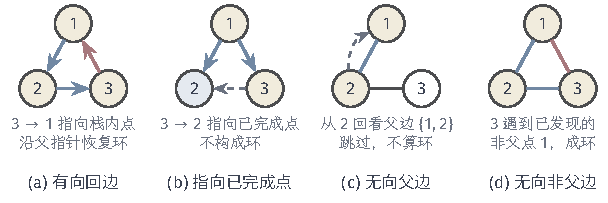
\includegraphics[width=102.9mm]{figures/01-basic-mathematics/04-graphs/tikz/c2-dfs-cycle-detection/figure.pdf}
  \caption{深度优先遍历中环的判断。黄色为处理中（在栈内）的顶点，蓝色填充为已完成顶点，蓝色粗线为父指针对应的边。(a)有向图中$3\to1$指向栈内顶点，构成回边，沿父指针恢复出环；(b)$3\to2$指向已完成顶点，不构成环；(c)无向图中从$2$回看父边$\{1,2\}$，这是同一条边的反向查看，应当跳过；(d)无向三角形中$3$遇到已发现、但不经父边相连的顶点$1$，构成环（红色）。}
  \label{fig:graph-trav-cycle-detection}
\end{figure}

\begin{theorem}[有向环的判定]
\label{thm:graph-trav-directed-cycle}
有限有向图含有向环，当且仅当对它的一次完整深度优先遍历中出现回边。出现回边$u\to v$时，父指针链$v\to\cdots\to u$加上弧$u\to v$就是一个有向环。
\end{theorem}

\begin{proof}
充分性已在上面说明：$v$处于处理中且$u$是当前栈顶，$u$在$v$上方，由引理~\ref{lem:graph-trav-dfs-nesting}$u$是$v$的后代，父指针链给出从$v$到$u$的有向路径。

必要性。设图含有向环，在环上取最先被发现的顶点$v$，记环上指向$v$的弧为$u\to v$。在时刻$d(v)$，环上其余顶点都未发现，沿环从$v$走到$u$的路径满足引理~\ref{lem:graph-trav-white-path}的条件，所以$u$成为$v$的后代，$d(v)<d(u)<f(u)<f(v)$。$u$在完成之前要检查弧$u\to v$，那时$v$尚未完成，仍处于处理中，因此$u\to v$是一条回边。
\end{proof}

\paragraph{无向图：跳过实际的父边}
无向图中每条边在两端的邻接表里各出现一次。从$u$走到$v$之后，$v$检查邻居时会再次看到$u$，这只是同一条边的反向记录，不是新的路线。若把它当作“遇到已发现顶点”，任何一条边都会被误判为环，如图~\ref{fig:graph-trav-cycle-detection}(c)。因此规则是：检查$u$的一条邻接记录$e=\{u,w\}$时，若$e$就是使$u$被发现的父边，跳过；否则只要$w$已经被发现，就报告存在环。图~\ref{fig:graph-trav-cycle-detection}(d)中，$3$经父边与$2$相连，它看到的$1$已被发现、且不经父边相连，于是$1\text{--}2\text{--}3\text{--}1$是一个环。允许平行边时，要按边的身份跳过，只跳过实际作为父边的那一条；两点之间的另一条平行边会与父边构成长度为$2$的环。

这一规则在两个方向上都可靠。若整次遍历从未报告，每条边在两端被检查时，要么发现了新顶点而成为父边，要么正是父边的反向记录，所以所有边都是父边，图就是深度优先森林本身，没有环。反过来，考察第一次报告时的边$e=\{u,w\}$，可以说明$w$此时一定在栈中。假设$w$已完成。$w$完成之前检查过$e$：若那时$u$未发现，$u$会成为$w$的后代并先于$w$完成，与$u$此刻仍在处理相矛盾；若那时$u$已发现，那次检查本身就该报告，除非$e$是$w$的父边，而这意味着$u$当初已经通过$e$发现了$w$，不会现在才第一次读到$e$。于是$w$是栈中位于$u$下方的祖先，父指针链从$w$到$u$再加上$e$构成一个环；由于$e$不是$u$的父边，在简单图中这个环至少有三个顶点。算法既给出了“有环”的结论，也给出了这个环本身，可以直接核对。

\section{连通结构的计算}
\label{sec:graph-connectivity-computation}

第~\ref{sec:graph-connectivity-separation}节把顶点按相互可达划分为连通分量或强连通分量，第~\ref{sec:graph-trees-forests}节说明每个无向分量都有生成树。这些都是存在性的定义。本节把它们算出来：先用遍历给无向图的每个分量编号并抽出生成森林；再处理边不断加入、分量不断合并的情形，引入并查集；最后计算有向图的强连通分量。后一个问题不能简单地重复启动遍历，因为从一个顶点出发能到达的范围，往往大于与它相互可达的范围。

\subsection{连通分量与生成森林}
\label{sec:graph-trav-components-forest}

\paragraph{外层扫描与分量编号}
一次广度或深度优先遍历恰好找出起点所在分量的全部顶点：在无向图中，可达关系是对称的，从$r$可达的顶点就是与$r$相互连通的顶点。要给所有分量编号，只需在外面再套一层扫描。

\begin{algorithm}[无向连通分量编号]
\label{alg:graph-trav-components}
输入：无向图的邻接表。输出：每个顶点的分量编号$\operatorname{comp}(v)$，以及分量数$c$。
\begin{enumerate}
  \item 所有顶点置为未标记，$c=0$。
  \item 按任意固定次序扫描顶点。遇到未标记的顶点$r$时，令$c\gets c+1$，从$r$启动一次广度（或深度）优先遍历，把这次新发现的每个顶点$v$标记为$\operatorname{comp}(v)=c$。已经标记的顶点不再作为起点，也不清除旧编号。
  \item 扫描完全部顶点后输出。
\end{enumerate}
\end{algorithm}

外层扫描必须覆盖全部顶点，否则没有边的孤立点永远不会被任何遍历发现，也就得不到编号。图~\ref{fig:graph-trav-components-forest}中的图由贯穿四点图、一条边$\{5,6\}$和孤立点$7$组成。按编号扫描，从$1$出发的遍历标出$\{1,2,3,4\}$；扫描到$2,3,4$时它们已有编号，跳过；从$5$出发标出$\{5,6\}$；最后$7$自成一个分量。若改变扫描次序，例如先扫描$7$，编号的数值会变，但哪些顶点被分到一起不会变，因为分量本身由图决定。各次遍历合起来把每个顶点和每条邻接记录处理常数次，总时间为$O(n+m)$。

\paragraph{保留发现父边得到生成森林}
遍历时每个新顶点都是经某条边第一次被发现的。把这些父边$\{p(v),v\}$全部保留下来，重复遇到已发现顶点的边一律不加，就得到原图的一个生成森林。

\begin{theorem}[发现父边构成生成森林]
\label{thm:graph-trav-parent-forest}
设对无向图$\mathcal G$执行算法~\ref{alg:graph-trav-components}，并保留所有父边。则这些父边与全部顶点组成$\mathcal G$的一个生成森林，它在每个分量上是一棵生成树，边数为$n-c$。
\end{theorem}

\begin{proof}
每个非起点顶点恰有一条父边，父边的另一端是更早发现的顶点；起点没有父边。于是父边共$n-c$条。

再说明父边不成环。假设某些父边构成一个环，取环上最晚发现的顶点$v$。$v$在环上有两条边，另两端都比$v$早发现。但与$v$相连的父边中，只有$v$自己的父边通向更早发现的顶点，其余父边都是$v$的子顶点的父边，另一端比$v$晚发现。矛盾。

最后，每次遍历从起点出发，沿父指针可以从任何新发现的顶点回到起点，所以每个分量内的父边是连通的。连通、无环、覆盖分量的全部顶点，就是该分量的生成树。
\end{proof}

\begin{figure}[!htb]
  \centering
  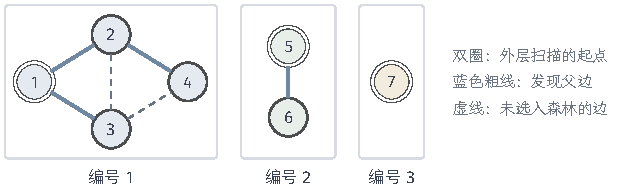
\includegraphics[width=104.8mm]{figures/01-basic-mathematics/04-graphs/tikz/c2-components-spanning-forest/figure.pdf}
  \caption{外层扫描与生成森林。图由贯穿四点图、边$\{5,6\}$和孤立点$7$组成，按编号扫描、每次启动广度优先遍历。三个分量分别获得编号$1,2,3$；双圈是每次遍历的起点，蓝色粗线是保留的父边，共$4=7-3$条，虚线边被检查过但未选入森林。}
  \label{fig:graph-trav-components-forest}
\end{figure}

\paragraph{生成森林丢掉了什么}
图~\ref{fig:graph-trav-components-forest}中第一个分量保留了$\{1,2\}$、$\{1,3\}$、$\{2,4\}$，舍弃了$\{2,3\}$和$\{3,4\}$。生成森林保留了“谁和谁连通”，却不保留其他结构。原图中$3$与$4$直接相邻，在森林中却要走$3\to1\to2\to4$三步；原图没有割点，删去任何一个顶点后其余顶点仍然连通，而在森林中删去$1$或$2$都会把树断开。此外，算法只关心是否连通，边上若有权重，选出的边也没有任何总权最小的保证；在所有生成树中选总权最小的一棵，是第~\ref{sec:graph-minimum-spanning-tree}节的问题。

\subsection{增量连通性与并查集}
\label{sec:graph-trav-union-find}

\paragraph{边不断加入时的分量}
设顶点集固定，边一条一条地加入，每加入一条边后都要回答“两个给定顶点现在是否连通”。每次都重新遍历全图需要$O(n+m)$时间，太浪费。注意加入边$\{u,v\}$对分量的影响很简单：若$u,v$原来已在同一分量，分量不变；否则把两个分量合并成一个。分量构成顶点集的一个划分，加边只会合并其中的两块，不会拆分。于是需要一种数据结构，维护若干互不相交的集合，支持两种操作：$\operatorname{find}(v)$返回$v$所在集合的代表元，两顶点连通当且仅当它们的代表元相同；$\operatorname{union}(u,v)$把$u$和$v$所在的两个集合合并。这种数据结构称为\term{并查集}（union-find），也称不相交集合结构。

\paragraph{父指针树}
并查集把每个集合存成一棵有根树：每个元素保存一个父指针，根的父指针指向自己，根就是集合的代表元。$\operatorname{find}(v)$从$v$出发沿父指针一直走到根；$\operatorname{union}(u,v)$先求出两个根，若不同，就把一个根的父指针改为指向另一个根。这里的父指针只表示“属于同一集合”，与原图的边没有关系：合并$\{1,3\}$时，可能是$3$的根被接到$1$的根下，而原图中这两个根之间未必有边。需要输出原图中的连接时，应另外保存实际加入的边。

\paragraph{按大小合并与路径压缩}
若合并时随意选择谁接到谁下面，树可能退化成一条长链，$\operatorname{find}$要走很多步。两条规则可以避免这一点。

\begin{algorithm}[并查集的两种操作]
\label{alg:graph-trav-union-find}
状态：每个元素$v$的父指针$\operatorname{parent}(v)$，每个根$r$所在集合的大小$\operatorname{size}(r)$。初始时每个元素自成一个集合，$\operatorname{parent}(v)=v$，$\operatorname{size}(v)=1$。
\begin{enumerate}
  \item $\operatorname{find}(v)$：沿父指针从$v$走到根$r$；然后把这条路上经过的每个元素的父指针都直接改为$r$（路径压缩）；返回$r$。
  \item $\operatorname{union}(u,v)$：求$r_u=\operatorname{find}(u)$、$r_v=\operatorname{find}(v)$。若$r_u=r_v$，不做任何事。否则把较小集合的根接到较大集合的根下，大小相同时把$r_v$接到$r_u$下（按大小合并），并把新根的大小更新为两者之和。
\end{enumerate}
\end{algorithm}

图~\ref{fig:graph-trav-union-find}按边序列$\{1,2\}$、$\{3,4\}$、$\{1,3\}$、$\{5,6\}$、$\{4,6\}$追踪这些操作。前两次合并各把一个单点接到另一个单点下，得到$\{1,2\}$与$\{3,4\}$，此时还有单点集合$\{5\}$、$\{6\}$。合并$\{1,3\}$时两个集合大小都是$2$，按约定把根$3$接到根$1$下，$4$的深度变为$2$。之后若查询$\operatorname{find}(4)$，沿$4\to3\to1$找到根$1$，路径压缩把$4$的父指针直接改为$1$，下次查询只需一步。合并$\{5,6\}$得到大小为$2$的集合；处理$\{4,6\}$时，$4$所在集合大小为$4$、$6$所在集合大小为$2$，于是根$5$接到根$1$下，全部六个元素属于同一集合。每一步后的集合划分都与“已加入的边构成的图的连通分量”一致。

\begin{figure}[!htb]
  \centering
  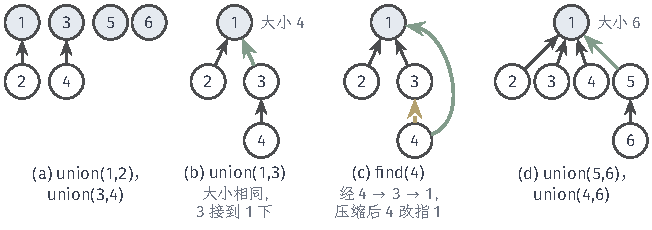
\includegraphics[width=110.5mm]{figures/01-basic-mathematics/04-graphs/tikz/c2-union-find/figure.pdf}
  \caption{并查集的父指针树，箭头由元素指向其父指针，蓝色填充为根。(a)合并$\{1,2\}$、$\{3,4\}$后；(b)合并两个大小为$2$的集合，按约定把根$3$接到根$1$下（绿色箭头）；(c)查询$\operatorname{find}(4)$经过$4\to3\to1$（黄色虚线是原父指针），路径压缩后$4$直接指向根$1$；(d)合并$\{5,6\}$后再处理$\{4,6\}$，较小集合的根$5$接到较大集合的根$1$下。}
  \label{fig:graph-trav-union-find}
\end{figure}

\paragraph{树高与操作开销}
按大小合并能保证树不会太高。

\begin{theorem}[按大小合并的树高]
\label{thm:graph-trav-union-by-size}
只使用按大小合并（无论是否路径压缩）时，任一元素到根的路径长度不超过$\log_2 n$，其中$n$是元素总数。
\end{theorem}

\begin{proof}
先不考虑路径压缩。一个元素的深度只在它所在的根被接到另一个根下面时增加$1$；按规则，被接的那一侧不大于另一侧，所以合并后该元素所在集合的大小至少是原来的两倍。集合大小从$1$开始，不超过$n$，至多翻倍$\log_2 n$次，深度也就至多为$\log_2 n$。路径压缩只把元素的父指针改为它的某个祖先，只会让深度变小，不影响这个上界。
\end{proof}

因此每次$\operatorname{find}$和$\operatorname{union}$都只需$O(\log n)$时间，存储为$O(n)$。路径压缩使反复查询同一区域变得更快。可以证明，两条规则同时使用时，任意$k$次操作的总时间为$O(k\,\alpha(n))$，其中$\alpha$是增长极慢的反Ackermann函数，对任何实际规模的$n$都不超过$4$；这一摊还分析较长，这里不展开，使用时只需记住每次操作的平均代价几乎是常数。

\paragraph{适用范围}
并查集适合“只加边、不删边”的情形。第~\ref{sec:graph-minimum-spanning-tree}节的Kruskal算法按边权从小到大考虑每条边，需要判断加入这条边是否会成环，也就是判断两个端点是否已在同一分量，正好用并查集完成。删除一条边可能把一个分量拆成两个，而并查集的合并无法撤销，所以它不能直接维护任意删边后的分量。在图像中给相连的像素区域编号时，也常先给像素临时标号、再用并查集合并相遇的标号，具体扫描方式留到应用部分。

\subsection{强连通分量与缩点}
\label{sec:graph-trav-scc}

\paragraph{一次搜索为什么不够}
在有向图中，从顶点$v$出发的一次遍历找到的是$v$能到达的全部顶点，而$v$所在的强连通分量要求双向可达。图~\ref{fig:graph-trav-kosaraju}(a)中，从$1$出发的深度优先遍历依次发现$1,2,3,4$，但$3,4$回不到$1$，$1$所在的强连通分量只是$\{1,2\}$。一般地，$v$所在的强分量等于“从$v$可达的顶点”与“能到达$v$的顶点”的交集；后者可以在把所有弧反向后的图上从$v$遍历得到。对每个顶点都这样做两次遍历需要$O(n(n+m))$时间。下面的算法只用两遍深度优先遍历，在$O(n+m)$时间内求出全部强连通分量。

\paragraph{两遍深度优先遍历}
把有向图$\mathcal G$的每条弧$u\to v$改为$v\to u$，得到\term{反向图}（reverse graph）$\mathcal G^{\mathrm{rev}}$。$\mathcal G$与$\mathcal G^{\mathrm{rev}}$的强连通分量相同，因为相互可达的两个顶点在弧全部反向后仍然相互可达。算法的第一遍在原图上计算完成时刻，第二遍在反向图上按完成时刻从大到小选择起点。这一方法称为\term{Kosaraju算法}（Kosaraju's algorithm）。

\begin{algorithm}[Kosaraju强连通分量算法]
\label{alg:graph-trav-kosaraju}
输入：有向图$\mathcal G=(V,E)$的出邻接表。输出：每个顶点所属强连通分量的编号。
\begin{enumerate}
  \item 在$\mathcal G$上执行完整的深度优先遍历（算法~\ref{alg:graph-trav-dfs}），覆盖全部顶点，记录完成次序。
  \item 扫描出邻接表，构造反向图$\mathcal G^{\mathrm{rev}}$的出邻接表，即原图的入邻接表。
  \item 所有顶点置为未标记。按完成时刻从大到小扫描顶点；遇到未标记的顶点$r$时，开始一个新分量，在$\mathcal G^{\mathrm{rev}}$上从$r$遍历（广度或深度优先均可），只进入未标记的顶点，把这次到达的顶点全部标为这个分量。
\end{enumerate}
\end{algorithm}

\paragraph{在三个强分量组成的图上追踪}
图~\ref{fig:graph-trav-kosaraju}的有向图有七个顶点，弧为$1\to2$、$2\to1$、$2\to3$、$3\to4$、$4\to3$、$5\to6$、$6\to4$、$6\to7$、$7\to1$、$7\to5$。它的强连通分量是$\{5,6,7\}$、$\{1,2\}$和$\{3,4\}$，分量之间只有单向的弧。

第一遍按编号选择起点、按编号读取出邻居。从$1$出发，依次发现$1,2,3,4$；$4$的出邻居$3$在栈中，$4$完成，随后$3,2,1$依次完成，完成时刻为$f(4)=5$、$f(3)=6$、$f(2)=7$、$f(1)=8$。接着从$5$重新出发，发现$5,6$；$6$的出邻居$4$已完成，跳过，再发现$7$；$7$的出邻居$1$已完成、$5$在栈中，于是$7,6,5$依次完成，$f(7)=12$、$f(6)=13$、$f(5)=14$。完成次序为$4,3,2,1,7,6,5$，见图~\ref{fig:graph-trav-kosaraju}(a)。

第二遍按完成时刻从大到小，即$5,6,7,1,2,3,4$选择起点，在反向图上遍历，见图~\ref{fig:graph-trav-kosaraju}(b)。从$5$出发，反向弧把它引向$7$，再引向$6$；$\{5,6,7\}$中没有反向弧通往别处，于是得到第一个分量$\{5,6,7\}$。下一个未标记的是$1$：反向弧$1\to2$、$1\to7$中$7$已标记，只进入$2$，得到$\{1,2\}$。最后从$3$出发，反向弧$3\to2$通往已标记的$2$，只进入$4$，得到$\{3,4\}$。每次遍历恰好停在一个强分量的边界上。若第二遍在原图而不是反向图上从$5$遍历，会经$6\to4$、$7\to1$走进另外两个分量，所以反向这一步不可省略。

\begin{figure*}[!htb]
  \centering
  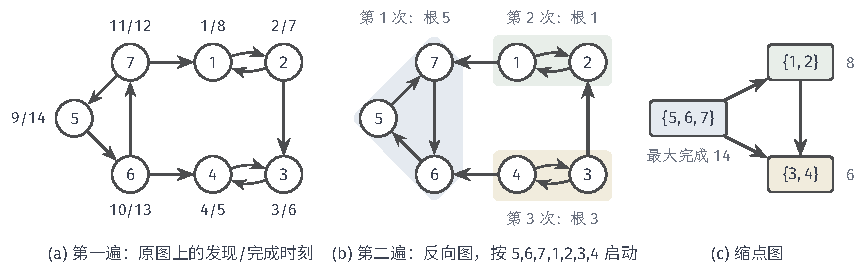
\includegraphics[width=146.5mm]{figures/01-basic-mathematics/04-graphs/tikz/c2-kosaraju-condensation/figure.pdf}
  \caption{Kosaraju算法的两遍过程与缩点图。(a)原图上按编号重启的深度优先遍历，顶点旁为发现/完成时刻；粗箭头是连接不同强分量的弧。(b)反向图上按完成时刻从大到小（$5,6,7,1,2,3,4$）选择起点，三次遍历分别得到蓝、绿、黄三个强连通分量，指向已标记分量的反向弧不再进入。(c)把每个强分量缩成一点得到的缩点图，旁注为各分量中最大的完成时刻；缩点图无环，且最大完成时刻沿弧方向递减。}
  \label{fig:graph-trav-kosaraju}
\end{figure*}

\paragraph{完成次序的性质}
第二遍之所以不会越界，是因为第一遍的完成时刻在分量之间有固定的先后。对强连通分量$C$，记$f(C)=\max_{v\in C}f(v)$为其中最大的完成时刻。在上例中，$f(\{5,6,7\})=14$、$f(\{1,2\})=8$、$f(\{3,4\})=6$，而分量之间的弧都从$f$值大的指向$f$值小的。

\begin{lemma}[分量间的完成时刻]
\label{lem:graph-trav-scc-finish}
设$C\neq C'$是有向图的两个强连通分量，且存在一条从$C$中顶点指向$C'$中顶点的弧。则在一次完整的深度优先遍历中，$f(C)>f(C')$。
\end{lemma}

\begin{proof}
考察$C\cup C'$中最先被发现的顶点$x$。

若$x\in C$。在时刻$d(x)$，$C\cup C'$中其余顶点都未发现。$C$中每个顶点都能从$x$经$C$内部的路径到达；$C'$中每个顶点都能先在$C$内走到那条弧的起点，经弧进入$C'$，再在$C'$内部到达。这些路径上的顶点此时都未发现，由引理~\ref{lem:graph-trav-white-path}，$C\cup C'$中其余顶点都成为$x$的后代并先于$x$完成，所以$f(C)=f(x)>f(C')$。

若$x\in C'$。同理，$C'$中其余顶点都成为$x$的后代，$f(C')=f(x)$。另一方面，从$C'$中的任何顶点都不能到达$C$：否则结合已有的从$C$到$C'$的弧，$C$与$C'$中的顶点相互可达，它们就应属于同一个强分量。所以在$x$处于处理中期间，$C$中没有顶点被发现（那样的顶点会是$x$的后代，从而从$x$可达）。$C$中顶点都在$f(x)$之后才被发现，也就在$f(x)$之后完成，所以$f(C)>f(x)=f(C')$。
\end{proof}

\paragraph{第二遍为什么恰好取出一个分量}
在反向图中，引理~\ref{lem:graph-trav-scc-finish}的不等式方向随弧一起反转：从分量$C$出发的反向弧只能通往$f$值更大的分量。第二遍按$f$值从大到小选择起点，这些分量在轮到$C$之前都已标记，于是遍历被挡在$C$之内。

\begin{theorem}[Kosaraju算法的正确性]
\label{thm:graph-trav-kosaraju}
算法~\ref{alg:graph-trav-kosaraju}第三步的每一次遍历，恰好标记一个强连通分量的全部顶点。
\end{theorem}

\begin{proof}
对第二遍已经完成的遍历次数归纳，假设此前每次遍历都恰好标记了一个完整的强分量。设下一个起点是$r$，所在分量为$C$。$r$是未标记顶点中完成时刻最大的；由归纳假设，未标记的顶点恰好组成若干个完整的强分量，所以$f(r)=f(C)$，且$C$在未标记的分量中$f$值最大。

$C$在反向图中仍然强连通，从$r$出发能到达$C$的全部顶点，而$C$中的顶点都未标记，因此都会被这次遍历标记。另一方面，设反向图中有一条弧从$C$中顶点指向另一个分量$C'$中的顶点，它对应原图中一条从$C'$指向$C$的弧，由引理~\ref{lem:graph-trav-scc-finish}有$f(C')>f(C)$。而$C$是未标记分量中$f$值最大的，所以$C'$已经被标记，这次遍历不会进入。因此这次遍历标记的恰好是$C$。
\end{proof}

\paragraph{计算开销}
第一遍深度优先遍历用$O(n+m)$时间。构造反向图需要扫描每条弧一次，时间与额外存储都是$O(n+m)$。第二遍按完成时刻从大到小扫描，只需把第一遍的完成次序倒过来读，不必排序；遍历本身再用$O(n+m)$时间。总时间为$O(n+m)$。三处细节缺一不可：第一遍必须覆盖全部顶点，否则有些顶点没有完成时刻；第二遍必须在反向图上进行；起点必须按完成时刻从大到小选择，若改为从小到大，上例中第二遍会先从$4$出发，在反向图上经$4\to6$进入$\{5,6,7\}$，再经$3\to2$进入$\{1,2\}$，把三个分量全部混在一起。

\paragraph{缩点图}
得到强连通分量后，可以把每个分量看成一个整体。把每个强分量压缩为一个顶点，若原图中有从分量$C$指向另一分量$C'$的弧，就在$C$与$C'$之间连一条弧$C\to C'$（多条这样的弧只保留一条，分量内部的弧舍去），得到的有向图称为\term{缩点图}（condensation graph）。图~\ref{fig:graph-trav-kosaraju}(c)中，缩点图有三个顶点和三条弧$\{5,6,7\}\to\{1,2\}$、$\{1,2\}\to\{3,4\}$、$\{5,6,7\}\to\{3,4\}$。

\begin{theorem}[缩点图无环]
\label{thm:graph-trav-condensation-dag}
任何有限有向图的缩点图都是有向无环图。
\end{theorem}

\begin{proof}
假设缩点图中有有向环$C_1\to C_2\to\cdots\to C_k\to C_1$，$k\geq2$，各$C_i$是不同的强分量。每条弧$C_i\to C_{i+1}$对应原图中一条从$C_i$中某顶点到$C_{i+1}$中某顶点的弧，而每个分量内部任意两点相互可达。于是从$C_1$中任一顶点出发，可以依次经过$C_2,\ldots,C_k$再回到$C_1$，环上所有分量中的顶点两两相互可达，它们应属于同一个强分量，与$C_1,\ldots,C_k$互不相同矛盾。
\end{proof}

由引理~\ref{lem:graph-trav-scc-finish}，缩点图中每条弧都从$f$值较大的分量指向$f$值较小的分量，所以Kosaraju算法第二遍得到分量的先后次序，恰好使缩点图的每条弧从先得到的分量指向后得到的分量。上例中得到的次序$\{5,6,7\}$、$\{1,2\}$、$\{3,4\}$就满足这一点。任何有向图都可以先缩点、再在无环的缩点图上安排先后，这正是下一节要研究的依赖排序。

\section{拓扑排序}
\label{sec:graph-topological-order}

编译程序时，一个模块要等它引用的模块编译完才能编译；计算一组中间量时，一个量要等它依赖的量算出来才能计算。用有向图表示这类依赖，弧$u\to v$表示$u$必须先于$v$处理，问题就是把所有顶点排成一列，使每条弧的起点都排在终点前面。

\begin{definition}[拓扑序]
\label{def:graph-trav-topological-order}
有向图$\mathcal G=(V,E)$的\term{拓扑序}（topological order）是$V$中全部顶点的一个排列$v_1,v_2,\ldots,v_n$，使得对每条弧$v_i\to v_j$都有$i<j$。求拓扑序的过程称为拓扑排序。
\end{definition}

拓扑序只要求每条弧前后正确，没有弧相连的两个顶点谁先谁后都可以，因此拓扑序一般不唯一。但并非每个有向图都有拓扑序。若图中有有向环$v_1\to v_2\to\cdots\to v_k\to v_1$，排列既要让$v_1$在$v_2$之前、$v_2$在$v_3$之前……$v_{k-1}$在$v_k$之前，又要让$v_k$在$v_1$之前，这不可能。所以有拓扑序的图一定没有有向环。下面的Kahn算法会证明反方向也成立，从而得到：

\begin{theorem}[拓扑序的存在性]
\label{thm:graph-trav-topological-existence}
有限有向图存在拓扑序，当且仅当它是有向无环图。
\end{theorem}

必要性已在上面说明；充分性由下面算法~\ref{alg:graph-trav-kahn}的正确性给出。本节给出两种构造拓扑序的方法，它们在遇到有向环时都会报告失败，而不是输出一个不完整的序列。

\subsection{Kahn算法}
\label{sec:graph-trav-kahn}

\paragraph{当前入度与零入度队列}
哪个顶点可以最先处理？没有任何依赖的顶点，也就是入度为$0$的顶点。把它输出后，它对后继的约束就满足了，可以把它和它的出弧从图中删掉；删掉之后，有些原来有依赖的顶点会变成入度为$0$，可以接着输出。实现时不必真的删除，只需维护每个顶点在“尚未输出的顶点构成的子图”中的当前入度，并用一个队列存放当前入度为$0$、尚未输出的顶点。这一方法称为\term{Kahn算法}（Kahn's algorithm）。

\begin{algorithm}[Kahn拓扑排序]
\label{alg:graph-trav-kahn}
输入：有向图$\mathcal G=(V,E)$的出邻接表。输出：一个拓扑序，或报告图中有有向环。
\begin{enumerate}
  \item 扫描全部弧，统计每个顶点的入度$\operatorname{indeg}(v)$。把所有入度为$0$的顶点（包括孤立点）放入队列$Q$，输出序列$L$置空。
  \item 当$Q$非空时，取出队首$u$，追加到$L$末尾。对每条出弧$u\to v$，令$\operatorname{indeg}(v)\gets\operatorname{indeg}(v)-1$；若它恰好降为$0$，把$v$放入$Q$。
  \item $Q$为空时停止。若$L$含全部$n$个顶点，输出$L$；否则报告有有向环。
\end{enumerate}
\end{algorithm}

一个顶点只在当前入度刚降到$0$的那一刻入队，因此不会重复入队。判断必须用当前入度，而不是初始入度：初始入度为$1$的顶点，在它唯一的前驱输出之前不能输出。

\paragraph{为什么总能找到零入度顶点}
算法能一直进行下去，依赖于下面的事实。

\begin{lemma}[有向无环图有源点]
\label{lem:graph-trav-dag-source}
非空的有限有向无环图至少有一个入度为$0$的顶点。
\end{lemma}

\begin{proof}
假设每个顶点的入度都至少为$1$。从任一顶点$v_0$出发，取它的一个前驱$v_1$，即有弧$v_1\to v_0$；再取$v_1$的一个前驱$v_2$，如此继续。顶点只有有限个，这个序列中必有某个顶点第二次出现，设$v_i=v_j$，$i<j$。则$v_j\to v_{j-1}\to\cdots\to v_i$是一个有向环，与无环矛盾。
\end{proof}

由此可以证明算法的正确性。在有向无环图上，尚未输出的顶点构成原图的诱导子图，删掉顶点不会产生新的环，它仍是有向无环图；只要它非空，由引理~\ref{lem:graph-trav-dag-source}就有当前入度为$0$的顶点，这个顶点已经在队列中。因此队列在全部顶点输出之前不会变空，$L$最终含全部$n$个顶点。对每条弧$u\to v$，$v$的当前入度要等$u$输出后才扣除这条弧的贡献，所以$v$只能在$u$之后入队、之后输出，$L$满足拓扑序的要求。这就证明了定理~\ref{thm:graph-trav-topological-existence}的充分性。

反过来，若图中有有向环，环上每个顶点在环上都有一个前驱，环上第一个被输出的顶点在输出之前当前入度至少为$1$，不可能入队，所以环上的顶点一个也不会输出，$L$少于$n$个顶点。这时已经输出的部分只是一个前缀，不能当作完整的拓扑序。若需要给出环本身，可以在剩下的顶点中重复引理~\ref{lem:graph-trav-dag-source}证明中的“不断取前驱”，必然在有限步内回到已经走过的顶点，找到一个有向环。

\paragraph{菱形依赖的入度变化}
考虑弧为$1\to2$、$1\to3$、$2\to4$、$3\to4$的菱形依赖：任务$2,3$都依赖$1$，任务$4$同时依赖$2$和$3$。初始入度为$(0,1,1,2)$，只有$1$入队。图~\ref{fig:graph-trav-kahn}(b)列出了每次输出后的变化。输出$1$后，$2,3$的入度都降为$0$，两者入队；输出$2$后，$4$的入度从$2$降为$1$，还不能入队；输出$3$后，$4$的入度降为$0$，入队；最后输出$4$。得到拓扑序$1,2,3,4$。

\begin{figure}[!htb]
  \centering
  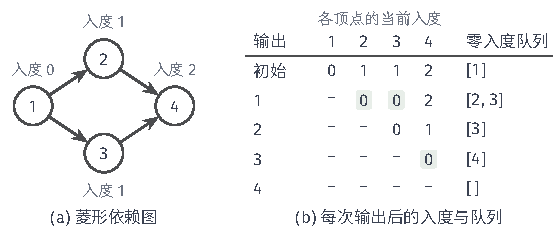
\includegraphics[width=94.8mm]{figures/01-basic-mathematics/04-graphs/tikz/c2-kahn-diamond/figure.pdf}
  \caption{Kahn算法在菱形依赖图上的执行。(a)依赖图及各顶点的初始入度。(b)每输出一个顶点后各顶点的当前入度（“--”表示已输出）与零入度队列；绿色底纹标出刚降为$0$、随即入队的入度。顶点$4$要等两个前驱都输出后才入队。}
  \label{fig:graph-trav-kahn}
\end{figure}

输出$1$之后，$2$和$3$同时位于队列中，这表示两项任务可以同时执行，或以任意先后执行。若先取$3$，就得到同样合法的$1,3,2,4$。队列中同时有多个零入度顶点时选哪一个，决定了得到哪个拓扑序。

\paragraph{计算开销}
统计入度要扫描每条弧一次；之后每个顶点入队、出队各一次，每条弧在其起点输出时被扣减一次。总时间为$O(n+m)$，入度数组、队列与输出序列占$O(n)$额外空间。若要求结果可复现，例如在多个零入度顶点中总是选编号最小的，就要把普通队列换成优先队列，每次入队、出队需要$O(\log n)$时间，总时间变为$O(m+n\log n)$。

\subsection{基于DFS的拓扑排序}
\label{sec:graph-trav-dfs-toposort}

\paragraph{逆完成次序}
第~\ref{sec:graph-trav-dfs-orders}节已经在一个例子中看到，把深度优先遍历的完成次序反转，弧的起点就排在了终点前面。下面说明这在无环图中总是成立。

\begin{theorem}[逆完成次序是拓扑序]
\label{thm:graph-trav-dfs-toposort}
对有向无环图执行一次覆盖全部顶点的深度优先遍历，则对每条弧$u\to v$都有$f(v)<f(u)$。因此按完成时刻从大到小排列顶点，得到一个拓扑序。
\end{theorem}

\begin{proof}
考察$u$检查弧$u\to v$的时刻，此时$u$处于处理中，按$v$的状态分三种情况。若$v$未发现，它将以$u$为父指针被发现，由引理~\ref{lem:graph-trav-dfs-nesting}，$f(v)<f(u)$。若$v$已完成，$f(v)$早于当前时刻，而$u$尚未完成，同样$f(v)<f(u)$。若$v$处于处理中，$u\to v$是一条回边，由定理~\ref{thm:graph-trav-directed-cycle}图中有有向环，与假设矛盾，这种情况不会发生。
\end{proof}

于是得到第二种构造：执行覆盖全部顶点的三色深度优先遍历；一旦遇到回边，就沿父指针返回一个有向环，拒绝输出排序；若始终没有回边，把完成次序反转后输出。实现时可以在每个顶点完成时把它放到输出序列的最前面，遍历结束时序列就已是逆完成次序。

\paragraph{与Kahn算法的结果比较}
在同一个菱形依赖图上，从$1$出发、按编号读取出邻居：发现$1,2,4$，$4$完成，$2$完成；回到$1$后发现$3$，$3$的出邻居$4$已完成，$3$完成；最后$1$完成。完成次序为$4,2,3,1$，反转得$1,3,2,4$，见图~\ref{fig:graph-trav-dfs-toposort}。它与Kahn算法给出的$1,2,3,4$不同，但两者都是合法拓扑序：把顶点按次序从左到右排开，四条弧全部指向右方。拓扑序可能不唯一，检验一个输出是否正确，标准是逐条弧核对先后，而不是与某一个特定答案比较。

\begin{figure}[!htb]
  \centering
  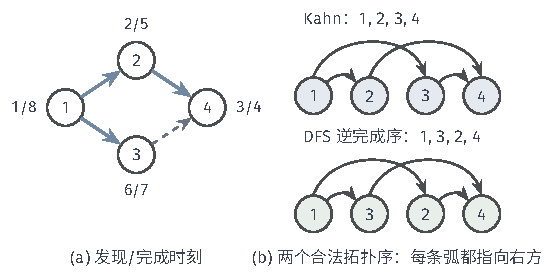
\includegraphics[width=93.8mm]{figures/01-basic-mathematics/04-graphs/tikz/c2-dfs-topological-order/figure.pdf}
  \caption{基于深度优先遍历的拓扑排序。(a)菱形依赖图上从$1$出发的深度优先遍历，旁注为发现/完成时刻，蓝色箭头为父指针对应的弧，虚线弧$3\to4$检查时$4$已完成。(b)Kahn算法得到的$1,2,3,4$与逆完成次序$1,3,2,4$，两种排列下每条弧都从左指向右，都是合法拓扑序。}
  \label{fig:graph-trav-dfs-toposort}
\end{figure}

\paragraph{必须覆盖全部顶点}
只从一个起点遍历时，得到的只是它可达部分的完成次序。在菱形图中若只从$2$出发，只能到达$2,4$，反转后是$2,4$，漏掉了$1$和$3$。也不能把各次重启的结果分别反转后简单拼接：先从$2$出发得到$2,4$，再从$1$出发得到$1,3$，拼成$2,4,1,3$，违反了弧$1\to2$。正确做法是把整次遍历的完成次序$4,2,3,1$作为一个整体反转，得到$1,3,2,4$；定理~\ref{thm:graph-trav-dfs-toposort}的证明对跨越不同起点的弧同样成立。

\paragraph{两种方法的选择}
两种方法的时间都是$O(n+m)$。Kahn算法显式地维护“当前可以执行的任务”这一集合，适合需要逐步列出可并行任务、或按某种优先规则选择任务的场合。基于深度优先遍历的方法不需要入度数组，在已经要做深度优先遍历、或需要在有环时给出环的场合可以直接复用同一次遍历。对一般有向图，可以先用第~\ref{sec:graph-trav-scc}节的方法求出强连通分量并缩点，再对无环的缩点图做拓扑排序。第~\ref{sec:graph-shortest-paths}节在有向无环图上计算最短路时，就是按拓扑序逐个处理顶点。

\section{基于分隔集的分块}
\label{sec:graph-separator-blocks}

大图上的计算常常希望“分而治之”：把图拆成几块分别处理，再在块与块的连接处汇总。第~\ref{sec:graph-connectivity-separation}节定义了分隔集：删除一个顶点集$S$后，若某些顶点之间不再有路径，$S$就把它们分隔开。本节接受一个给定的候选集$S$，用连通分量计算检验它是否真的把图拆成了几侧，再把$S$加回各侧，得到共享接口的局部块。本节只负责结构上的分块：怎样找到好的分隔集不在这里讨论，块上的数值怎样沿接口组合则放在第~\ref{chap:graph-dynamic-programming}章。

\subsection{删除集合后的分量}
\label{sec:graph-trav-delete-separator}

\paragraph{输入、输出与三种结果}
输入是无向图$\mathcal G=(V,E)$和一个候选集合$S\subseteq V$。删除$S$中的顶点及与它们关联的边，得到$\mathcal G-S$，即$V\setminus S$上的诱导子图；对它计算连通分量$C_1,\ldots,C_r$。不同的$C_j$之间在$\mathcal G-S$中没有边，所以原图中从$C_j$到$C_k$（$j\neq k$）的任何路径都必须经过$S$。按$r$的取值有三种结果：$r\geq2$时，$S$把图拆成了$r$侧，任取两个不同分量中的顶点，$S$都把它们分隔开；$r=1$时，删除$S$后其余顶点仍然连通，$S$没有形成多侧拆分；$r=0$时$S=V$，余图为空，也谈不上拆分。是否拆分成功只能由计算结果判断，不能因为输入被称作“分隔集”就默认成立。

\begin{algorithm}[删除候选集后的分量]
\label{alg:graph-trav-separator-components}
输入：无向图的邻接表，候选集合$S\subseteq V$。输出：$\mathcal G-S$的连通分量$C_1,\ldots,C_r$，以及拆分是否成功（$r\geq2$）。
\begin{enumerate}
  \item 用一个布尔数组标记$S$中的顶点为“屏蔽”，不修改原邻接表。
  \item 对未屏蔽的顶点执行算法~\ref{alg:graph-trav-components}：外层扫描跳过屏蔽顶点，遍历时读到屏蔽的邻居一律跳过。
  \item 输出各分量；若$r\geq2$报告拆分成功，$r=1$报告未拆分，$r=0$报告余图为空。
\end{enumerate}
\end{algorithm}

\paragraph{贯穿图上的检验}
在贯穿四点图上取$S=\{2,3\}$。删除$2,3$后，与它们关联的边$\{1,2\}$、$\{1,3\}$、$\{2,3\}$、$\{2,4\}$、$\{3,4\}$全部消失，只剩顶点$1$和$4$，而$\{1,4\}$不是原图的边，所以余图有两个分量$\{1\}$与$\{4\}$，见图~\ref{fig:graph-trav-separator-blocks}(a)。$S=\{2,3\}$成功地分隔了$1$和$4$。作为对照，取$S=\{1\}$，删除后剩下的$2,3,4$两两相邻，构成一个三角形，余图只有一个分量，见图~\ref{fig:graph-trav-separator-blocks}(c)，$\{1\}$不是有效的拆分。贯穿图中删去任何单个顶点都不会断开余图：删去$1$或$4$剩下三角形，删去$2$或$3$剩下一条路径，所以它没有割点，至少要删两个顶点才能拆开。

\paragraph{检验与优化是两个问题}
上面的计算回答的是“这个给定的$S$是否拆开了图”，用$O(n+m)$时间就能完成。它不回答“最小的拆分集合是什么”。若想通过检验来找最小的分隔集，就要逐个尝试候选集合：大小为$k$的候选集有$\binom{n}{k}$个，每个都要做一次连通分量计算，规模稍大就无法承受。寻找小的分隔集需要另外的方法，它们不是一次连通标记能自动给出的。

\subsection{局部块与公共接口}
\label{sec:graph-trav-blocks-interfaces}

\paragraph{把接口加回各侧}
删除$S$之后，各分量之间不再相连；但原图中分量内的顶点与$S$之间的边、$S$内部的边也随之丢失了。要把原图完整地分成几块，需要把$S$加回每一侧，得到\term{局部块}（local block）
\[
\mathcal B_j=\mathcal G[C_j\cup S],\qquad j=1,\ldots,r,
\]
其中$S$称为各块的公共接口。图~\ref{fig:graph-trav-separator-blocks}(b)中两个局部块是$\mathcal G[\{1,2,3\}]$与$\mathcal G[\{2,3,4\}]$，都是三角形，共享顶点$2,3$和边$\{2,3\}$。

\begin{figure}[!htb]
  \centering
  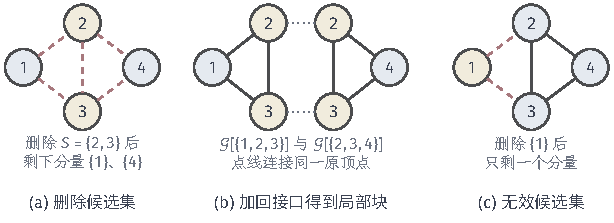
\includegraphics[width=103.9mm]{figures/01-basic-mathematics/04-graphs/tikz/c2-separator-blocks/figure.pdf}
  \caption{基于分隔集的分块。黄色顶点为候选删除集，红色虚线为随之删去的边。(a)贯穿四点图删除$S=\{2,3\}$后剩下两个分量$\{1\}$与$\{4\}$；(b)把$S$加回各侧得到两个局部块，两块中的$2,3$是同一批原顶点（点线相连），边$\{2,3\}$被两块共同引用；(c)删除$\{1\}$后余下三角形仍然连通，没有形成拆分。}
  \label{fig:graph-trav-separator-blocks}
\end{figure}

局部块覆盖了原图的每一条边。原图的一条边有三种可能：两端都在某个$C_j$中，或一端在$C_j$、一端在$S$中，这两种边都属于$\mathcal B_j$；两端都在$S$中，这样的边属于每一个块。由于不同分量之间没有边，不存在第四种情况。因此，原图的全部信息都保存在这些块中，块与块之间只通过$S$发生联系。

\paragraph{共享引用与复制}
不同局部块中的接口顶点是同一批原顶点，而不是可以各自独立变化的副本。若以后要给顶点赋值，同一个接口顶点在各块中必须取相同的值；若块中记录了边的数据，$S$内部的边被多个块同时看到，汇总时不能重复计数。因此表示局部块时，应保存接口顶点和接口边的唯一身份，各块只引用它们，而不是把原图的一部分真正复制几份后各自修改。

\paragraph{计算与存储开销}
屏蔽$S$并计算余图分量需要$O(n+m)$时间。输出局部块的存储另计：各块顶点数之和为$\sum_j(|C_j|+|S|)=(n-|S|)+r|S|$，接口顶点被重复列出$r$次；$S$内部的边也在每个块中出现一次。$r$和$|S|$都较小时，这部分额外存储可以忽略；接口很大或块很多时，就应采用共享引用。

\paragraph{小接口不保证块内简单}
接口小，只说明块与块之间的联系少，并不说明每个块内部简单。例如两个各有$100$个顶点的完全图只共用一个顶点，删除这个顶点就把图拆成两侧，接口大小为$1$，可每个局部块仍是一个$100$个顶点的完全图。分块的收益取决于后续计算在块内需要做什么。第~\ref{chap:graph-dynamic-programming}章会看到，当计算由许多只涉及少数顶点的局部项组成时，固定接口上的取值后各块可以分别处理，这时接口大小直接决定中间表的规模；那里还会把一次分块推广为多层的树分解。

\section{顶点标记与结构比较}
\label{sec:graph-wl-refinement}

第~\ref{sec:graph-isomorphism}节把两个图同构定义为存在保持邻接的顶点双射，并指出顶点数、边数、度分布等必要条件一般不足以判定同构。直接尝试所有$n!$个双射又不可行。本节介绍一种折中的办法：给每个顶点一个标记，然后反复根据“自己是什么、邻居都是什么”更新标记，使结构上不同的顶点逐渐得到不同的标记。这些标记不依赖顶点的编号，可以用来比较两个图；但我们也会看到，它并不能区分所有不同构的图。

\subsection{邻域标记与多重集合}
\label{sec:graph-trav-neighborhood-labels}

\paragraph{从度数到邻居的类别}
无属性的图里，顶点一开始没有任何可区分的信息，可以给所有顶点同一个初始标记；带属性的图则可以把属性作为初始标记。记顶点$i$的初始标记为$c_i^{(0)}$。第一步自然的细化是看邻居个数，即度数：三点路径$1\text{--}2\text{--}3$中，两个端点各有一个邻居，中点有两个邻居，于是端点与中点被区分开。更进一步，不只数邻居有几个，还要看邻居分别属于哪一类、每类有几个。这样，“有两个端点邻居的顶点”和“有一个端点邻居、一个中点邻居的顶点”也能被区分。

\paragraph{多重集合}
怎样记录“邻居都属于哪些类、各几个”？普通集合不行：两个邻居都是$A$类时，集合$\{A,A\}$就是$\{A\}$，丢失了次数。按顶点编号排出邻居标记的序列也不行：同一个顶点的邻居换一种编号，序列的次序就变了，而我们要的信息不应依赖编号。合适的对象是\term{多重集合}（multiset）：它像集合一样不计次序，又像序列一样记录每个元素出现的次数。用双花括号表示多重集合，例如$\{\!\{A,A,B\}\!\}$含两个$A$、一个$B$，它不等于$\{\!\{A,B\}\!\}$，但等于$\{\!\{A,B,A\}\!\}$。实际比较两个多重集合时，可以先把元素排序，再逐项比较。

\paragraph{签名与统一编码}
把顶点自己的旧标记与邻居标记的多重集合放在一起，称为该顶点在第$t$轮的签名：
\[
\sigma_i^{(t)}=\Bigl(c_i^{(t)},\ \{\!\{c_j^{(t)}:j\in N(i)\}\!\}\Bigr).
\]
签名完全由图的结构和当前标记决定，与顶点编号无关。比较两个图时，两图必须使用同一种初始标记规则，并且把签名翻译成新标记时使用同一本“字典”：同一个签名在两个图中必须得到同一个新标记。否则即使两图结构相同，标记的名称也可能对不上。

还要注意，不能为了“容易区分”而给每个顶点附上唯一的编号作为初始标记。那样所有顶点一开始就互不相同，比较的就不再是无属性图的结构，而是“编号也必须对应”的另一个问题。只有当属性本身是图的数据、并随顶点重编号一起移动时，才把它作为初始标记，这时比较的是带属性的图。

\subsection{1-WL标记细化}
\label{sec:graph-trav-wl-algorithm}

\paragraph{同步细化的规则}
有了签名，更新规则就是：所有顶点同时计算签名，签名相同的顶点得到相同的新标记，签名不同的得到不同的新标记。

\begin{definition}[1-WL标记细化]
\label{def:graph-trav-wl-refinement}
给定无向图$\mathcal G=(V,E)$与初始标记$c_i^{(0)}$，对$t=0,1,2,\ldots$同步计算
\begin{equation}
c_i^{(t+1)}=\operatorname{enc}\bigl(\sigma_i^{(t)}\bigr)
=\operatorname{enc}\Bigl(c_i^{(t)},\ \{\!\{c_j^{(t)}:j\in N(i)\}\!\}\Bigr),
\qquad i\in V,
\label{eq:graph-trav-wl-update}
\end{equation}
其中$\operatorname{enc}$是单射，即不同的签名映为不同的新标记。这一过程称为一维Weisfeiler--Leman标记细化（1-WL），也称\term{颜色细化}（color refinement）。第$t$轮的标记把$V$划分为若干类，记为$\mathcal P^{(t)}$。
\end{definition}

“同步”是指第$t+1$轮的所有签名都只读取第$t$轮的标记：先为全部顶点算完签名，再统一替换。若边算边替换，后处理的顶点会读到一部分新标记、一部分旧标记，结果就依赖处理次序，从而依赖编号。$\operatorname{enc}$的单射要求是数学上的约定；实际程序常用哈希函数把签名压缩成整数，而不同签名可能碰巧得到相同的哈希值。所以实现时应当比较完整的签名，或用字典给每个新出现的签名分配一个新整数，不能只凭哈希值判定两个签名相等。

\paragraph{三点路径上的细化}
图~\ref{fig:graph-trav-wl-path}从三点路径$1\text{--}2\text{--}3$开始，初始标记全为$A$。第$0$轮的签名为：端点$1,3$是$(A,\{\!\{A\}\!\})$，中点$2$是$(A,\{\!\{A,A\}\!\})$。两种签名不同，分别编码为$B$与$C$，得到$c^{(1)}=(B,C,B)$，划分为$\{1,3\}$、$\{2\}$。第$1$轮的签名为：端点是$(B,\{\!\{C\}\!\})$，中点是$(C,\{\!\{B,B\}\!\})$，编码为$D$与$E$，得到$c^{(2)}=(D,E,D)$。标记的名称换了，但划分仍是$\{1,3\}$、$\{2\}$，与上一轮相同，细化到此停止。

\begin{figure}[!htb]
  \centering
  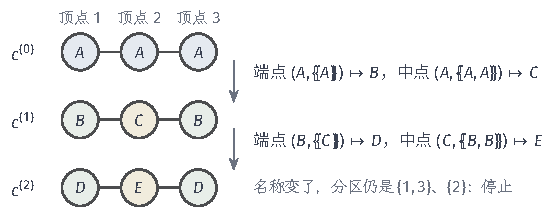
\includegraphics[width=94.0mm]{figures/01-basic-mathematics/04-graphs/tikz/c2-wl-path-refinement/figure.pdf}
  \caption{三点路径上的1-WL标记细化。每行是一轮标记，颜色表示所属的类；右侧是由签名得到新标记的编码。第一轮把端点与中点分开；第二轮标记名称改变，但划分仍为$\{1,3\}$、$\{2\}$，细化停止。}
  \label{fig:graph-trav-wl-path}
\end{figure}

\paragraph{只拆分不合并，有限轮后停止}
上例显示，判断停止要看划分，而不是看标记的名称。下面的引理说明划分只会越来越细，并且一旦某轮没有变化，以后也不会再变。

\begin{lemma}[1-WL的单调性与停止]
\label{lem:graph-trav-wl-refine}
对定义~\ref{def:graph-trav-wl-refinement}中的划分：（1）$\mathcal P^{(t+1)}$是$\mathcal P^{(t)}$的细分，即第$t+1$轮同类的顶点在第$t$轮也同类；（2）若$\mathcal P^{(t+1)}=\mathcal P^{(t)}$，则以后各轮划分都不再改变；（3）至多$n-1$轮严格细分后，划分就停止变化。
\end{lemma}

\begin{proof}
（1）若$c_i^{(t+1)}=c_j^{(t+1)}$，由$\operatorname{enc}$是单射得$\sigma_i^{(t)}=\sigma_j^{(t)}$，签名的第一个分量相等，即$c_i^{(t)}=c_j^{(t)}$。

（2）两轮划分相同，意味着存在标记之间的一一对应$\varphi$，使得对每个顶点$c_i^{(t+1)}=\varphi(c_i^{(t)})$。把$\varphi$作用到签名的每个分量上，得到$\sigma_i^{(t+1)}=\bigl(\varphi(c_i^{(t)}),\{\!\{\varphi(c_j^{(t)}):j\in N(i)\}\!\}\bigr)$。$\varphi$是一一对应，所以$\sigma_i^{(t+1)}=\sigma_k^{(t+1)}$当且仅当$\sigma_i^{(t)}=\sigma_k^{(t)}$，即$c_i^{(t+2)}=c_k^{(t+2)}$当且仅当$c_i^{(t+1)}=c_k^{(t+1)}$。因此$\mathcal P^{(t+2)}=\mathcal P^{(t+1)}$，依此类推。

（3）每次严格细分至少使类的个数加一，类的个数从至少$1$开始、不超过$n$，所以严格细分至多$n-1$次。由（2），第一次没有变化之后就再也不会变化。
\end{proof}

\paragraph{计算开销}
每一轮要为每个顶点读取全部邻居的标记，共$O(n+m)$次读取；把顶点$i$的邻居标记排序成多重集合的规范形式需要$O(d_i\log d_i)$时间；再把全部签名排序或查字典以分配新标记。一轮的总代价为$O((n+m)\log n)$量级。由引理~\ref{lem:graph-trav-wl-refine}，至多$n$轮就能确认划分稳定（最后一轮用于确认没有变化），所以总时间不超过$O(n(n+m)\log n)$。实际图上细化往往在少数几轮内稳定，总开销远小于这个上界。

\subsection{判别能力与局限}
\label{sec:graph-trav-wl-power}

\paragraph{在不交并上比较两个图}
要用1-WL比较图$\mathcal G_1$与$\mathcal G_2$，把两图放在一起看成一个不交并，用同一个初始标记规则和同一本字典同步细化，然后在每一轮分别统计两图中每种标记出现的次数。这种比较方法称为\term{一维Weisfeiler--Leman检验}（1-dimensional Weisfeiler--Leman test）。若某一轮两图的计数不同，就可以断定两图不同构；若计数在细化稳定前始终相同，只能说这一方法没有区分它们。

为什么计数不同就能断定不同构？设$\pi$是从$\mathcal G_1$到$\mathcal G_2$的同构，且初始标记满足$c_{\pi(i)}^{(0)}=c_i^{(0)}$（无属性时所有初始标记相同，自然满足；有属性时同构本来就要求保持属性）。$\pi$把$i$的邻居一一映为$\pi(i)$的邻居，对轮数归纳可得$\sigma_{\pi(i)}^{(t)}=\sigma_i^{(t)}$，于是$c_{\pi(i)}^{(t+1)}=c_i^{(t+1)}$。$\pi$是顶点之间的双射，每种标记在两图中的出现次数就相同。同样的推理说明，对同一个图重新编号顶点（用第~\ref{sec:graph-isomorphism}节的置换表示），各顶点的标记随之移动，标记计数不变：1-WL的结果不依赖编号，也不依赖图的画法。

例如，四个顶点的路径与四个顶点的星形都有$4$个顶点、$3$条边。初始标记全为$A$时，第一轮路径得到两个“一个邻居”的端点和两个“两个邻居”的内点，星形得到三个“一个邻居”的叶和一个“三个邻居”的中心，计数不同，两图不同构。这一轮区分的其实就是度分布，更多轮次则会区分邻居的度、邻居的邻居的度，等等。

\paragraph{六环与两个三角形}
1-WL的判别能力是有限的。图~\ref{fig:graph-trav-wl-limitation}中，六个顶点的环与两个不相连的三角形都有$6$个顶点、$6$条边，每个顶点的度都是$2$。初始标记全为$A$时，每个顶点的签名都是$(A,\{\!\{A,A\}\!\})$，所有顶点得到同一个新标记；下一轮又是同样的情形。标记从第一轮起就稳定为一类，两图的计数始终相同，1-WL无法区分它们。可是它们并不同构：六环是连通的，而两个三角形构成两个连通分量。用第~\ref{sec:graph-trav-components-forest}节的方法数一下连通分量，就能立刻把它们分开。

\begin{figure}[!htb]
  \centering
  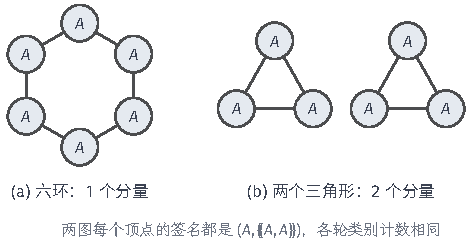
\includegraphics[width=79.5mm]{figures/01-basic-mathematics/04-graphs/tikz/c2-wl-cycle-triangles/figure.pdf}
  \caption{1-WL的局限。(a)六顶点环与(b)两个不相连的三角形初始标记全为$A$；每个顶点在每一轮都看到两个同类邻居，签名恒为$(A,\{\!\{A,A\}\!\})$，两图各轮的标记计数完全相同。两图分量数不同，并不同构。}
  \label{fig:graph-trav-wl-limitation}
\end{figure}

这个例子说明了1-WL的本质：每个顶点只能看到以自己为中心、逐轮向外扩大的邻域中“各类邻居有几个”，而六环和三角形上的每个顶点，无论看多少轮，看到的局部情形都一样。连通分量数这种整体性质，局部的计数无法反映。因此1-WL计数不同可以作为不同构的证据，计数相同则不能作为同构的证明。实践中常把它与分量数、环长等其他检验结合使用，各种检验互为补充；要确认同构，仍需给出一个实际的保持邻接的双射并逐边核对。

\section{本章小结}
\label{sec:graph-traversal-summary}

本章的出发点是：第~\ref{chap:graph-objects}章定义的可达、分量、无环和同构，怎样在一张实际的图上算出来。回答的共同方式是沿邻接表有组织地访问顶点，用少量状态记住已经知道的东西，而不去枚举路径或双射。表~\ref{tab:graph-trav-summary}对照了本章各方法所维护的状态、输出和计算时间。

\begin{table*}[!htb]
  \centering
  \caption{本章方法维护的状态、输出与时间。时间均以邻接表存储计，$n$为顶点数，$m$为边数或弧数。}
  \label{tab:graph-trav-summary}
  \small
  \begin{tabular}{@{}llll@{}}
    \toprule
    方法 & 维护的状态 & 输出 & 时间 \\
    \midrule
    广度优先遍历 & 队列、距离、父指针 & 最少边数与一条最短路线 & $O(n+m)$ \\
    深度优先遍历 & 三色状态、栈帧、时刻 & 发现次序、完成次序、回边 & $O(n+m)$ \\
    分量编号 & 外层扫描、分量号 & 连通分量、生成森林 & $O(n+m)$ \\
    并查集 & 父指针树、集合大小 & 加边过程中的分量代表 & 每次$O(\log n)$ \\
    Kosaraju算法 & 完成次序、反向图 & 强连通分量、缩点图 & $O(n+m)$ \\
    Kahn算法 & 当前入度、零入度队列 & 拓扑序或有环报告 & $O(n+m)$ \\
    分隔集分块 & 屏蔽标记、分量号 & 余图分量、局部块 & $O(n+m)$ \\
    1-WL细化 & 各轮标记、签名字典 & 稳定划分、标记计数 & 每轮$O((n+m)\log n)$ \\
    \bottomrule
  \end{tabular}
\end{table*}

这些输出回答的是不同的问题。广度优先遍历的层数回答“离起点最少几步”，深度优先遍历的完成次序回答“谁的后续全部探完”，它在无环图上给出拓扑序，在一般有向图上把强连通分量按缩点图的先后分离出来。并查集的代表元回答“在已加入的边下是否连通”，1-WL的标记回答“局部邻域在计数意义下是否一样”。同一张图上，这些量可以同时计算，但不能互相替代：深度优先的父路径不是最短路线，发现次序不是拓扑序，并查集的父指针不是原图的边，1-WL计数相同也不是同构的证明。

判断一个算法的输出是否正确，标准是看它是否满足相应的结构条件，而不只是看算法是否停止。广度优先遍历的父路径应恰有$d(v)$条边；生成森林应有$n-c$条边且无环；拓扑序应使每条弧从前指向后；有环报告应附带一个可以逐弧核对的环；强连通分量在第二遍中不应越过已标记的分量；分块检验应报告余图实际有几个分量。各节的定理正是把这些条件与算法的状态联系起来的依据。

本章得到的可达区域、生成森林和依赖次序，都只描述了“能否连接、按什么次序”，没有比较不同路线或不同边集的代价：广度优先遍历只数边数，生成森林只保证连通。下一章在这些可行结构的基础上引入边上的数值，研究最短路、最小生成树、最大流、最小费用流和匹配；本章的并查集用于Kruskal算法，拓扑序用于有向无环图上的最短路递推。第~\ref{chap:graph-dynamic-programming}章则沿着第~\ref{sec:graph-separator-blocks}节的接口思想，把局部块上的计算组织起来。

